\section{The aLIGO Input Mode Cleaner}

LIGO interferometers use several high finesse optical cavities for gravitational wave detection. The lengths of these cavities are controlled using radio frequency (RF) modulation-demodulation techniques in a Pound-Drever-Hall (PDH) locking scheme. This scheme provides a PDH error signal that is linear to cavity length over a specific range. This study examines the specific case of the triangular ring cavity uses in LIGO interferometers for input mode cleaning. When the length of the cavity approaches the boundaries of the PDH error signal linear range, our model of the input mode cleaner PDH response shows that the resulting error signal contains non-linear spectral artifacts. This model and understanding of the non-linear cavity responses will be useful in the commissioning phase of the Advanced LIGO project for more precisely locating and eliminating systematic noise sources in the interfereometers

\section{Modeling the IMC PDH loop}

The PDH response of the cavity was modeled using measured values of optical reflectivity and free spectral range of the Livingston input mode cleaner. The input beam was the nominal LIGO carrier beam with a frequency of $\omega = 281.8$ THz ($\lambda = 1064$ nm) and modulation sidebands of $\Omega = \pm24$ MHz.

The reflection coefficient of a LIGO input mode cleaner as a function of input beam frequency is given as,

\begin{equation}
F(\omega) = \frac{r(1 + e^{-i\phi})}{1+r^2e^{-i\phi}} = \frac{r(1 + e^{-i(\frac{\omega}{\nu_{fsr}})})}{1+r^2e^{-i(\frac{\omega}{\nu_{fsr}})}}
\end{equation}

where $r$ is the reflectivity of the input mirror, $\phi$ is the round-trip phase accumulated when traversing the cavity, and $\nu_{fsr}$ is the free spectral range of the cavity \cite{Mueller}.

In a situation where the carrier beam is resonant in the cavity and the modulation sidebands are high enough in frequency that they are not resonant, the PDH error signal, here denoted $\epsilon$ is given as

\begin{equation}
\epsilon(\omega) = -2\sqrt{P_{c}P_{s}}\operatorname{Im}\{F(\omega)F^*(\omega + \Omega) - F^*(\omega)F(\omega - \Omega)\},
\end{equation}

where $P_{c}$ is the the carrier beam power and $P_{s}$ is the sideband power \cite{Black01}.

Note: the above error signal is a function of laser frequency. This is an artifact of the original intent of PDH locking: using a fixed length resonant cavity to control the frequency of a laser by forcing it to match the cavity length. We can apply the same technique but flip the direction of feedback and use a highly stable laser to control the length of a free swinging resonant cavity by pushing on the mirrors to match the cavity length to the laser wavelength. The laser frequency detuning and cavity length detuning are linearly mapped to one another using the free spectral range of the resonant cavity.

Importantly, this error signal is linear to the length of the IMC within a certain range of motion. If the optics begin swinging too far away from the nominal locking point, we will begin to see a non-linear response and eventually a lock loss.

To explore this non-linearity, we injected a sinusoidal cavity motion into our model and observed the resulting error signal.

We explored two specific cases. Figure 1 shows spectra of the injected sinusoidal cavity motion (green) and the resulting non-linear error signal (blue). This motion was injected asymetrically about the nominal cavity locking point ($\epsilon = 0$) and therefore we see both even and odd harmonics of the injection frequency.

Figure 2 shows spectra of the injected sinusoidal cavity motion (green) and the resulting non-linear error signal (blue). However, this time the motion was injected symetrically about the nominal cavity locking point and as a result we only see odd harmonics of the fundamental frequency.

We hope to use this model as an explanation of systematic noise found in the aLIGO IMC.

\begin{figure}[h!]
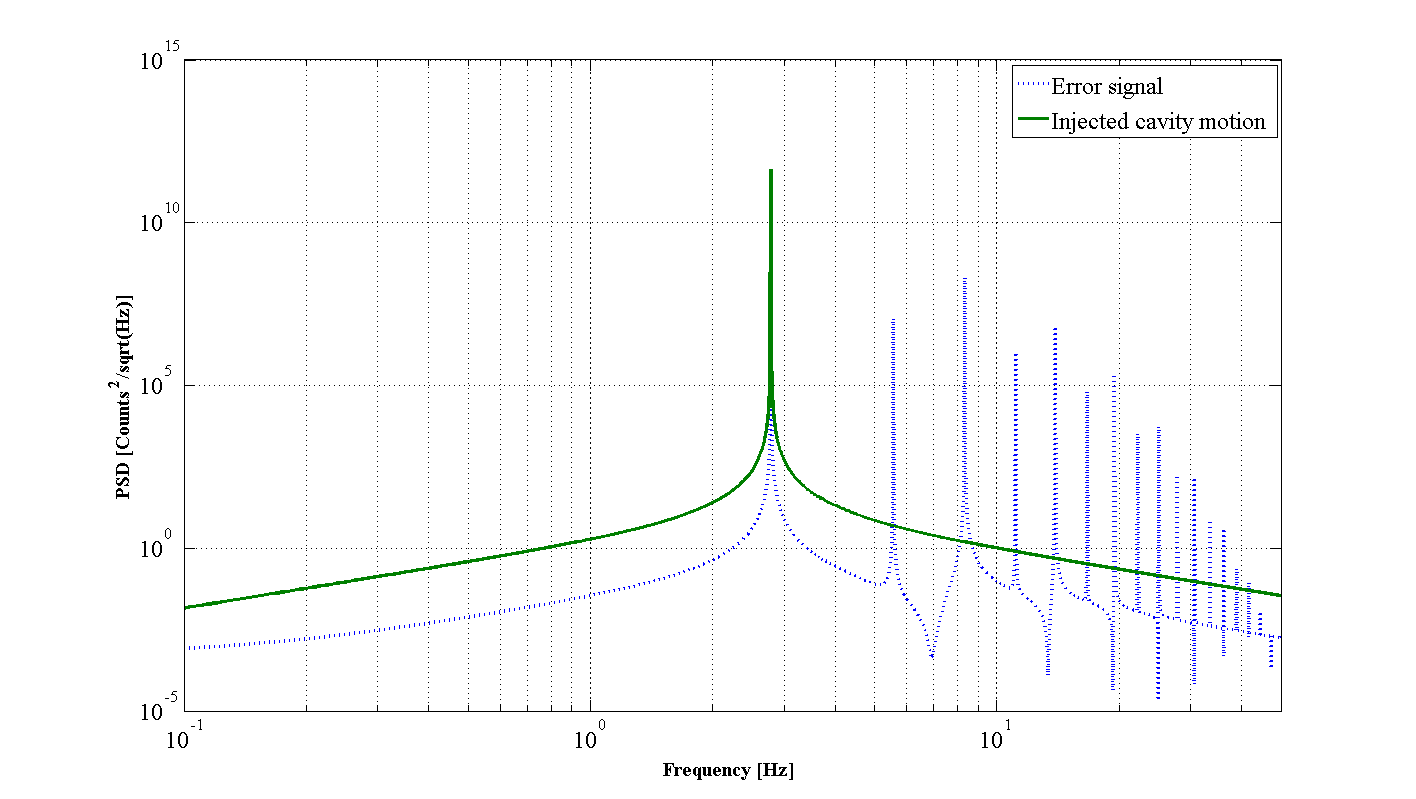
\includegraphics[height=0.6\textwidth]{figures/IMCUpconversion/PDH_error_signal_harmonics.png}
\caption[PDH response to asymmetric cavity motion]{Sinusoidal cavity motion with frequency 2.78 Hz injected asymmetrically about the locking point of the cavity results in a PDH error signal containing non-linear spectral artifacts at harmonics of the injected cavity motion.}
\end{figure}

\begin{figure}[h!]
\caption[PDH response to symmetric cavity motion]{If the motion is symmetric about the cavity locking point, we see only odd harmonics of the injection frequency.}
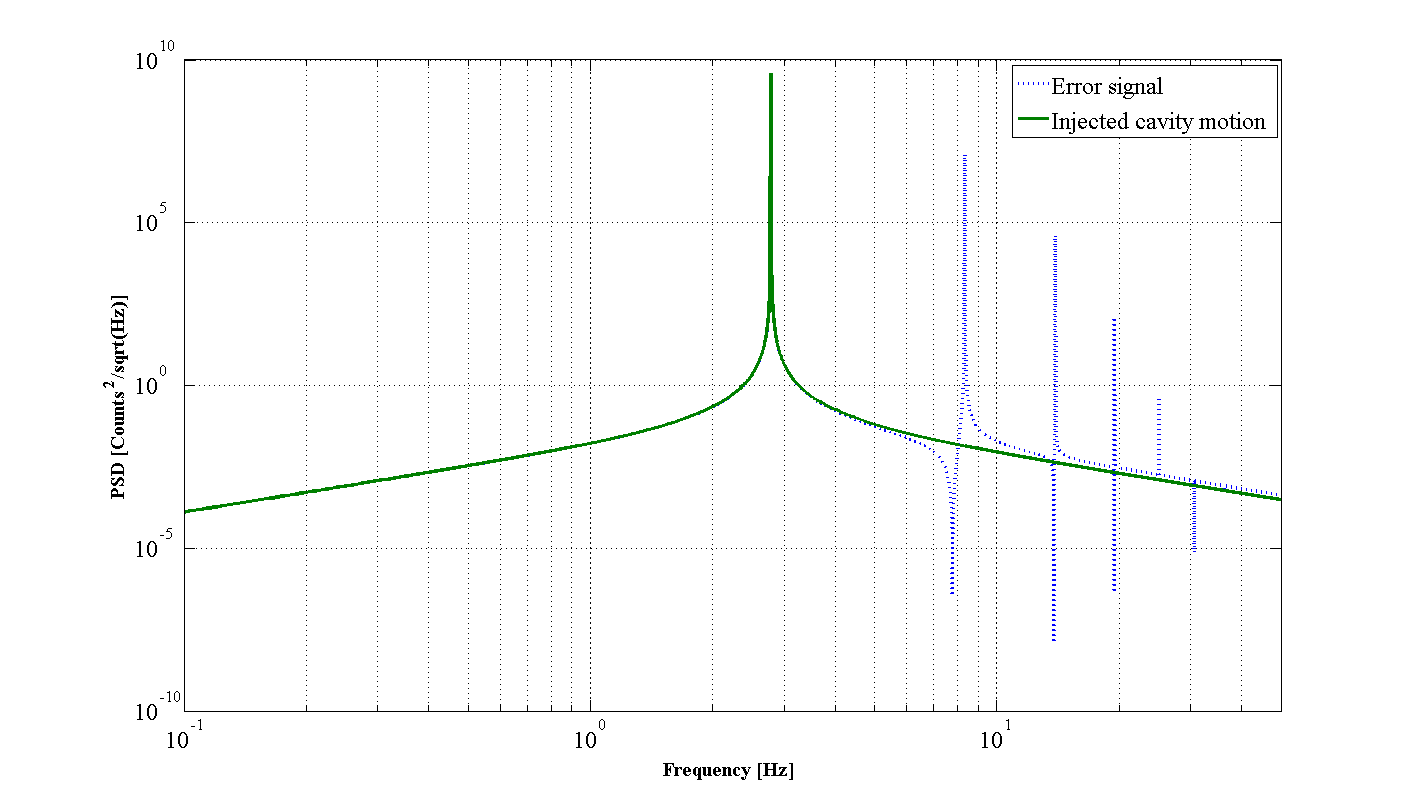
\includegraphics[height=0.6\textwidth]{figures/IMCUpconversion/symmetric_PDH.png}
\end{figure}

\section{Upconversion noise in aLIGO}
The aLIGO input mode cleaner (IMC) is a triangular ring cavity whose length is sensed and controlled using the PDH locking technique. Each of the three mirrors in the cavity is staged as the bottom mass of a triple suspension in order to passively isolate the mirrors from  potential noise sources. In addition, the chambers holding the IMC mirrors are isolated from ground motion by two stages of active seismic isolation. This isolation, however, is not completely impervious to external excitations. During periods of time with excess ground motion we can see seismic noise coupling into the cavity length and its control signal.

Specifically, when we see excess seismic noise in the 1-5 Hz anthropogenic band (believed to be caused by a commercial railroad a few kilometers from the LIGO Livingston Laboratory), we see highly structured noise in the IMC control signal in the 10-100 Hz band. This physical mechanism is consistent with the idea of a PDH range saturation. If excess seismic motion reaches the suspension and the optics begin swinging around, it's feasible that they could start to saturate the linear range of the PDH loop.

The noise takes a form very similar in structure to the non-linear PDH signal, displaying strong odd harmonics and weaker even harmonics. The IMC control signal has an associated noise floor that obscures parts of these peaks. The theoretical model uses sinusoids with a highly specified frequency and thus displays very sharp peaks in its spectrum. It should be noted that the peaks in the IMC control signal are the manifestation of a physical process, not digitally generated, and have some natural width to them.

\begin{figure}[h!]
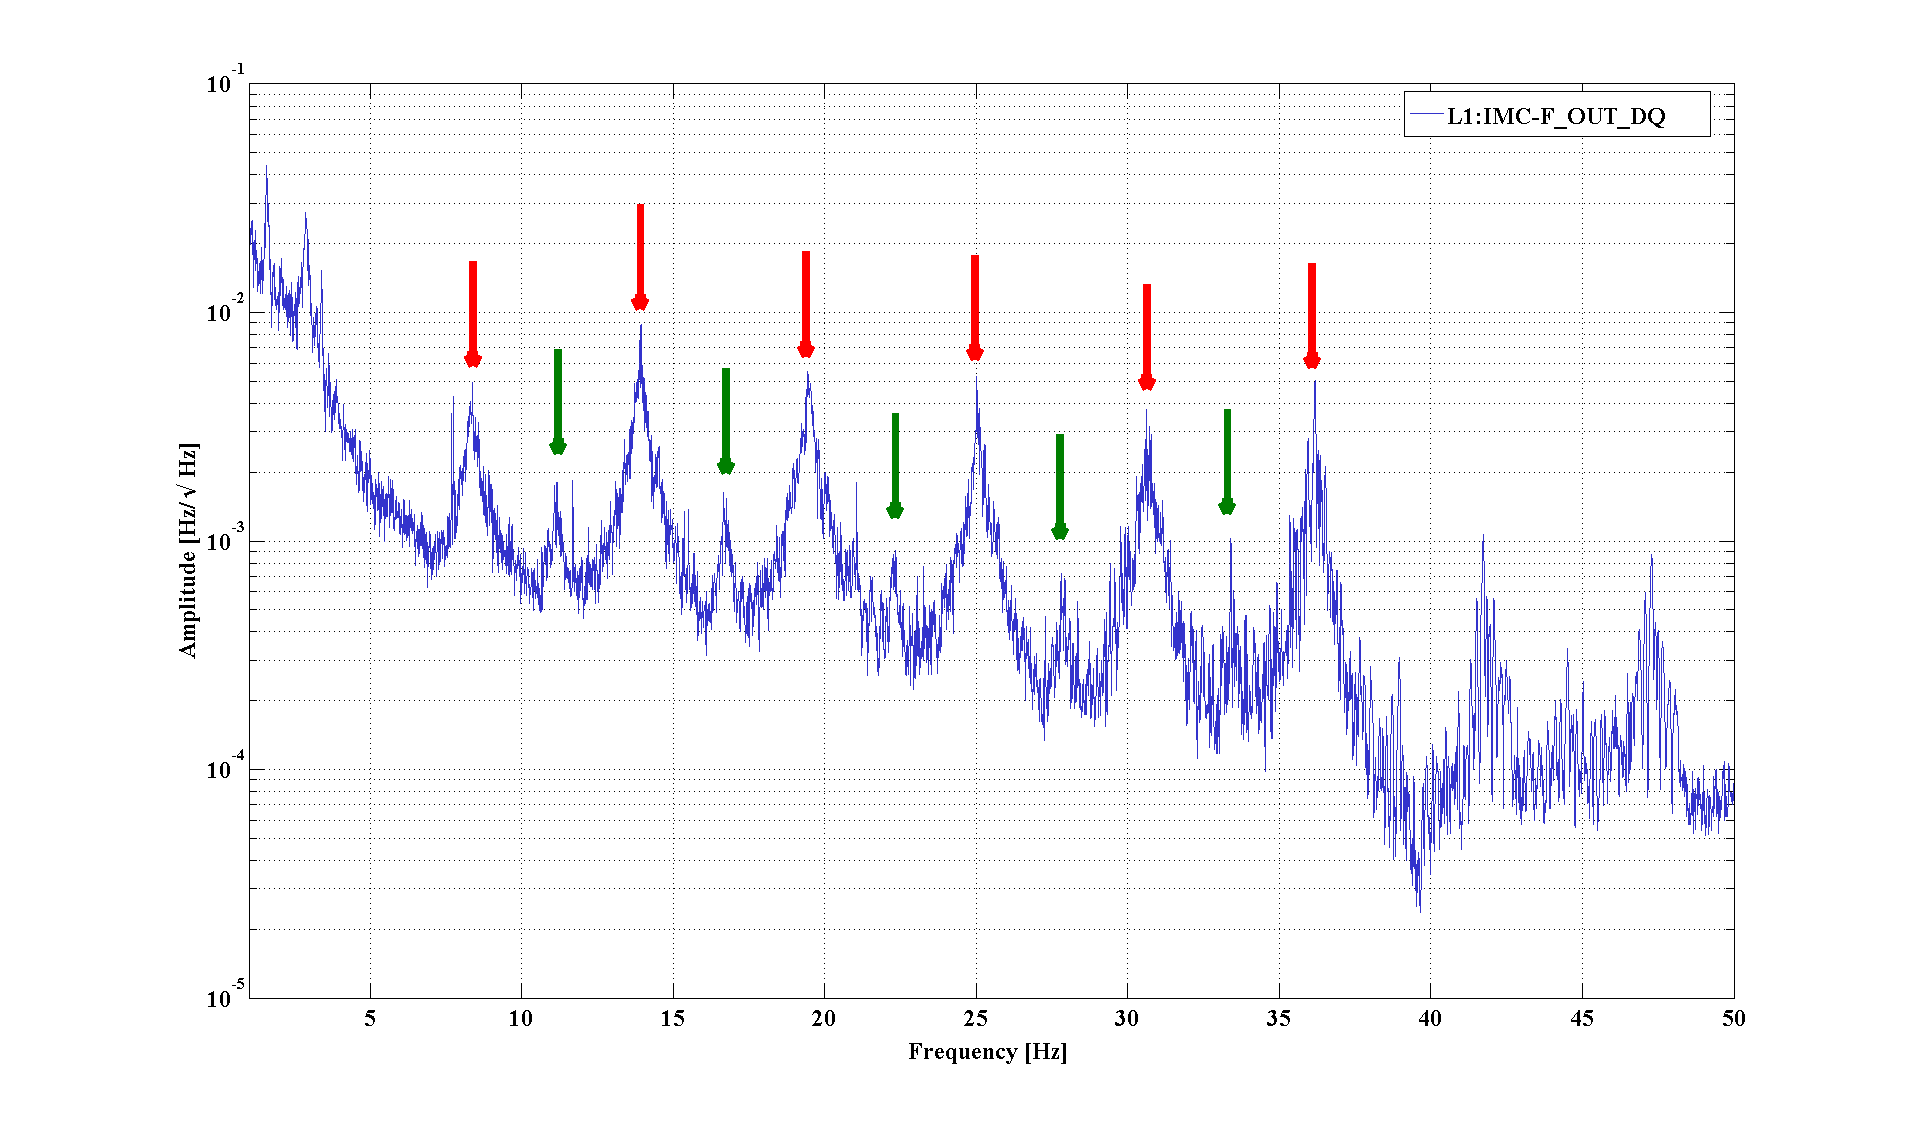
\includegraphics[height=0.6\textwidth]{figures/IMCUpconversion/upconversion_comb.png}
\caption[Spectral comb in IMC control signal]{Spectral comb with a fundamental frequncy of 2.78 Hz in the IMC control signal. Red arrows indicate odd harmonics, green arrows indicate even harmonics. }
\end{figure}

While we have demonstrated that this mechanism is a feasible explanation for the IMC upconversion noise, it has not yet been fully proven. We are currently looking for a better way to look at the actual IMC error point during times of excess seismic motion instead of the control signal. 

We also need to localize the source of the 2.78 Hz excitation. Why that specific frequency when the excess seismic noise is spread across a 1 - 5 Hz band? We think the source may be a vertical resonance of the triple pendulum suspension that houses the IMC optics being rung up by the excess motion.

We are also going to use the increasing full IFO uptime to figure out whether or not this upconversion noise is coupling downstream into critical cavities such as the recycling or arm cavities.

\section{Conclusions}

We found that injecting sinusoidal cavity motion into our input mode cleaner PDH model generates an error signal with non-linear spectral artifacts, specifically harmonics of the injection frequency, if the cavity motion exceeds the linear PDH range. For cavity motion that is symmetric about the locking point of the error signal, we find that the error signal contains only odd harmonics. For asymmetric cavity motion we find both even and odd harmonics, where the odd harmonics are typically higher in amplitude. In such a case, the amplitude of the even harmonics increases as the DC offset from the nominal locking point increases, that is, as the cavity motion is more asymmetric.

